\documentclass{article}

\usepackage{fancyhdr}
\usepackage{extramarks}
\usepackage{amsmath}
\usepackage{amsthm}
\usepackage{amsfonts}
\usepackage{tikz}
\usepackage[plain]{algorithm}
\usepackage{algpseudocode}
\usepackage[shortlabels]{enumitem}
\usepackage{mathtools}
\usepackage{amssymb}
\usepackage{hyperref}
\usepackage{tikz}
\usepackage{pgfplots}

\usetikzlibrary{automata,positioning}

%
% Basic Document Settings
%

\topmargin=-0.45in
\evensidemargin=0in
\oddsidemargin=0in
\textwidth=6.5in
\textheight=9.0in
\headsep=0.25in

\linespread{1.1}

\pagestyle{fancy}
\lhead{\hmwkAuthorName}
\chead{\hmwkClassTime (\hmwkClassInstructor): \hmwkTitle}
\lfoot{\lastxmark}
\cfoot{\thepage}

\renewcommand\headrulewidth{0.4pt}
\renewcommand\footrulewidth{0.4pt}

\setlength\parindent{0pt}

%
% Create Problem Sections
%

\newcommand{\enterProblemHeader}[1]{
    \nobreak\extramarks{}{Problem \arabic{#1} continued on next page\ldots}\nobreak{}
    \nobreak\extramarks{Problem \arabic{#1} (continued)}{Problem \arabic{#1} continued on next page\ldots}\nobreak{}
}

\newcommand{\exitProblemHeader}[1]{
    \nobreak\extramarks{Problem \arabic{#1} (continued)}{Problem \arabic{#1} continued on next page\ldots}\nobreak{}
    \stepcounter{#1}
    \nobreak\extramarks{Problem \arabic{#1}}{}\nobreak{}
}

\setcounter{secnumdepth}{0}
\newcounter{partCounter}
\newcounter{homeworkProblemCounter}
\setcounter{homeworkProblemCounter}{1}
\nobreak\extramarks{Problem \arabic{homeworkProblemCounter}}{}\nobreak{}

\newcommand{\hmwkTitle}{Problem Set 4}
\newcommand{\hmwkDueDate}{April 12, 2024}
\newcommand{\hmwkClass}{Introduction to Economics}
\newcommand{\hmwkClassTime}{ECON 101}
\newcommand{\hmwkClassInstructor}{Robert McDonough}
\newcommand{\hmwkAuthorName}{\textbf{Rushil Umaretiya}}

%
% Title Page
%

\title{
    \vspace{2in}
    \textmd{\textbf{\hmwkClass:\ \hmwkTitle}}\\
    \normalsize\vspace{0.1in}\small{\textbf{Due\ on\ \hmwkDueDate\ at 11:59pm}}\\
    \normalsize\text{Tuesday/Thursday 3:30-4:45, Genome Sciences 100}\\
    \vspace{0.1in}\large{\textit{\hmwkClassInstructor\ - \hmwkClassTime}}
    \vspace{3in}
}

\author{\hmwkAuthorName\\\small{rumareti@unc.edu}}
\date{}

\renewcommand{\part}[1]{\textbf{\large Part \Alph{partCounter}}\stepcounter{partCounter}\\}

%
% Various Helper Commands
%

% Useful for algorithms
\newcommand{\alg}[1]{\textsc{\bfseries \footnotesize #1}}

% For derivatives
\newcommand{\deriv}[1]{\frac{\mathrm{d}}{\mathrm{d}x} (#1)}

% For partial derivatives
\newcommand{\pderiv}[2]{\frac{\partial}{\partial #1} (#2)}

% Integral dx
\newcommand{\dx}{\mathrm{d}x}

% Alias for the Solution section header
\newcommand{\solution}{\textbf{\large Solution}}

\newcommand{\question}[1]{\pagebreak\section{Question #1}}

% Probability commands: Expectation, Variance, Covariance, Bias
\newcommand{\E}{\mathrm{E}}
\newcommand{\Var}{\mathrm{Var}}
\newcommand{\Cov}{\mathrm{Cov}}
\newcommand{\Bias}{\mathrm{Bias}}

\begin{document}

\maketitle

\question{1}

Use the AD-AS model to forecast how the economy will respond to
each of the following scenarios. For each scenario (1) indicate whether
AD or AS will shift, and in which direction; (2) draw a graph illustrating how the economy will respond in the short-run; (3) characterize
what the short-run equilibrium means for the economy (e.g., will it
create inflation, a recession, etc.)

\begin{enumerate}[(a)]
    \item Due to rapid economic development in India, Ford pickup trucks produced in America become very popular and exports rise.
    
    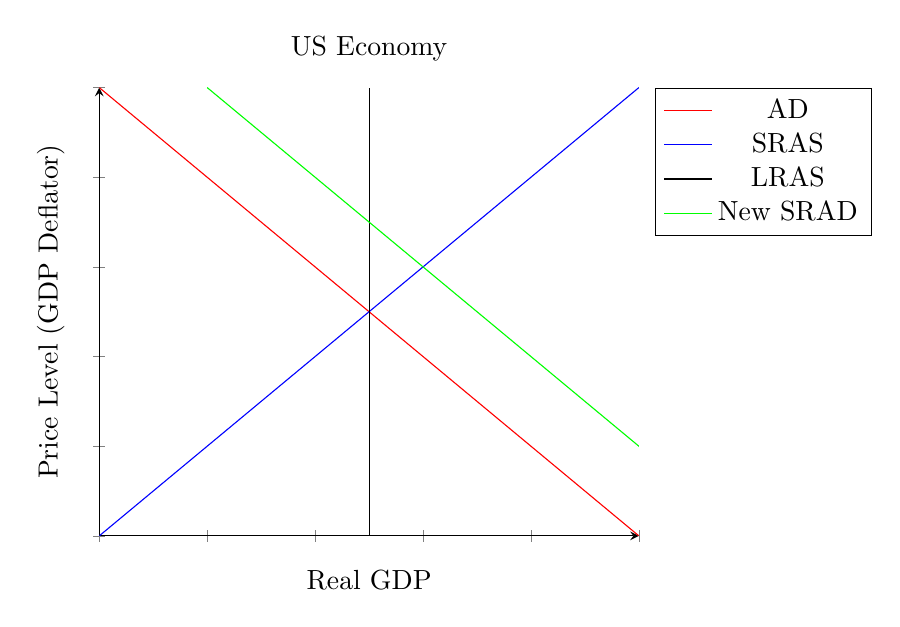
\begin{tikzpicture}
        \begin{axis}[
            title={US Economy},
            ylabel={Price Level (GDP Deflator)},
            xlabel={Real GDP},
            xmin=0, xmax=100,
            ymin=0, ymax=100,
            yticklabels={,,},
            xticklabels={,,},
            axis lines=left,
            grid=none,
            legend pos=outer north east,
        ]

        \addplot[
            color=red,
            ]
            coordinates {
            (0,100)(100,0)
            };
        \addlegendentry{AD}


        \addplot[
            color=blue,
            ]
            coordinates {
            (0,0)(100,100)
            };

        \addlegendentry{SRAS}

        \addplot[
            color=black,
            ]
            coordinates {
            (50,0)(50,100)
            };
        \addlegendentry{LRAS}

        \addplot[
            color=green,
            ]
            coordinates {
            (20,100)(120,0)
            };
        \addlegendentry{New SRAD}

        \end{axis}
    \end{tikzpicture}

    Due to a surge in exports, the aggregate demand curve shifts to the right. This will lead to an increase in the price level and real GDP causing increased inflation and economic growth.

    \item A computer virus is released that targets automated industrial machinery, severely limiting the amount of production by American manufacturing firms for about 2 months.
    
    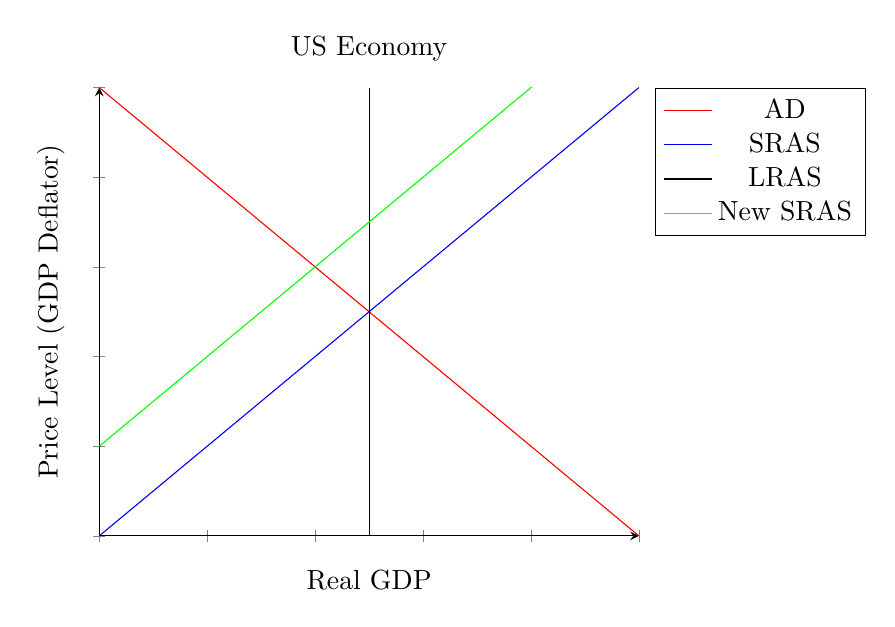
\begin{tikzpicture}
        \begin{axis}[
            title={US Economy},
            ylabel={Price Level (GDP Deflator)},
            xlabel={Real GDP},
            xmin=0, xmax=100,
            ymin=0, ymax=100,
            yticklabels={,,},
            xticklabels={,,},
            axis lines=left,
            grid=none,
            legend pos=outer north east,
        ]

        \addplot[
            color=red,
            ]
            coordinates {
            (0,100)(100,0)
            };
        \addlegendentry{AD}


        \addplot[
            color=blue,
            ]
            coordinates {
            (0,0)(100,100)
            };

        \addlegendentry{SRAS}

        \addplot[
            color=black,
            ]
            coordinates {
            (50,0)(50,100)
            };
        \addlegendentry{LRAS}

        \addplot[
            color=green,
            ]
            coordinates {
            (0,20)(100,120)
            };
        \addlegendentry{New SRAS}

        \end{axis}
    \end{tikzpicture}

    Due to a decrease in production, the short-run aggregate supply curve shifts to the left. This will lead to a decrease in real GDP and an increase in the price level causing a recession and inflation.

    \item In 2017 President Trump signed a tax bill that reduced income taxes for many Americans. Now, in 2023, some of those tax cuts are expiring, meaning that income taxes for Americans may go up in 2024.
    

    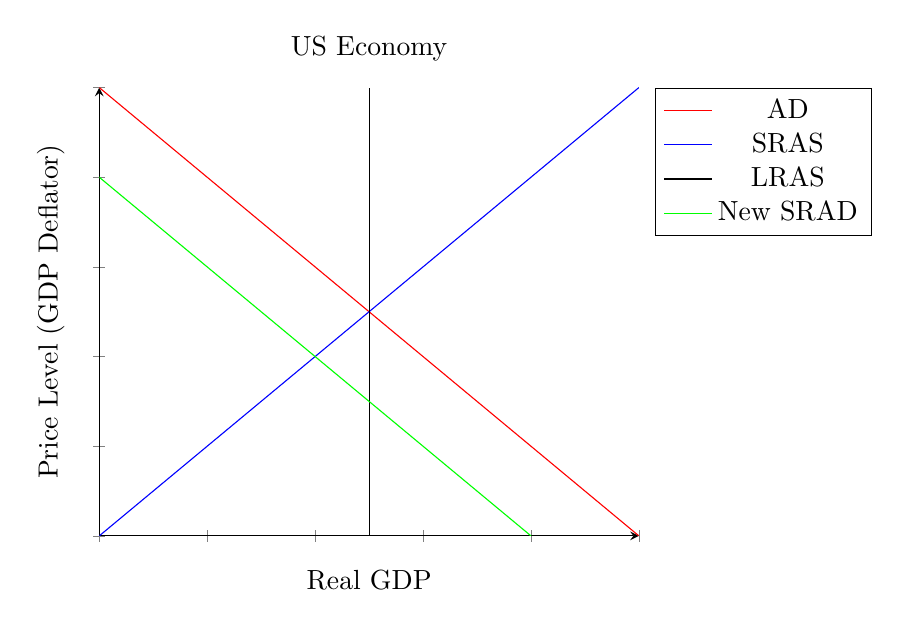
\begin{tikzpicture}
        \begin{axis}[
            title={US Economy},
            ylabel={Price Level (GDP Deflator)},
            xlabel={Real GDP},
            xmin=0, xmax=100,
            ymin=0, ymax=100,
            yticklabels={,,},
            xticklabels={,,},
            axis lines=left,
            grid=none,
            legend pos=outer north east,
        ]

        \addplot[
            color=red,
            ]
            coordinates {
            (0,100)(100,0)
            };
        \addlegendentry{AD}


        \addplot[
            color=blue,
            ]
            coordinates {
            (0,0)(100,100)
            };

        \addlegendentry{SRAS}

        \addplot[
            color=black,
            ]
            coordinates {
            (50,0)(50,100)
            };
        \addlegendentry{LRAS}

        \addplot[
            color=green,
            ]
            coordinates {
            (-20,100)(80,0)
            };
        \addlegendentry{New SRAD}

        \end{axis}
    \end{tikzpicture}

    Due to an increase in income taxes, the aggregate demand curve shifts to the left. This will lead to a decrease in the price level and real GDP causing a recession and deflation.

    \item With the new GDP report, American businesses become more confident that a recession is not approaching, and the economic expansion is likely to continue for the foreseeable future.
    
    
    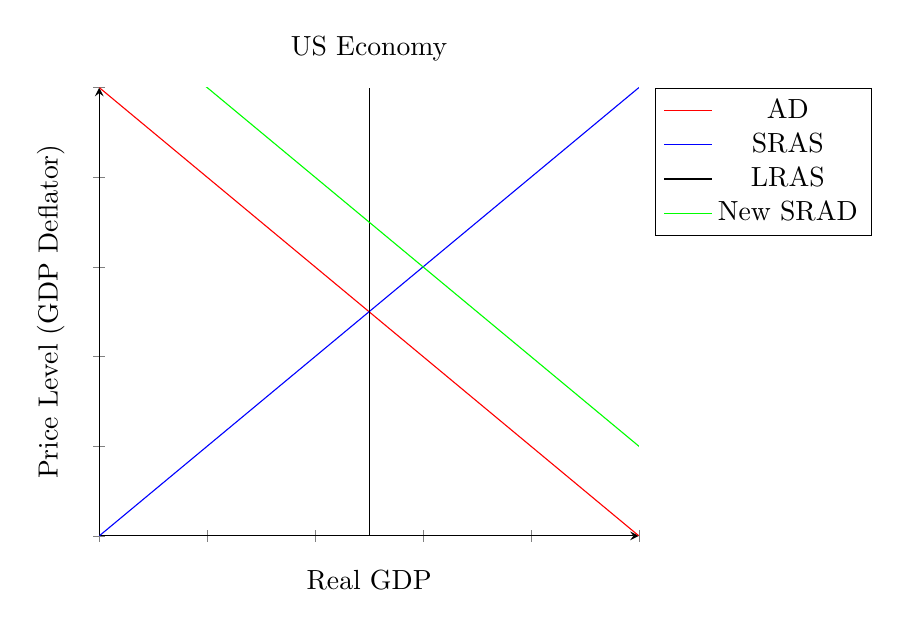
\begin{tikzpicture}
        \begin{axis}[
            title={US Economy},
            ylabel={Price Level (GDP Deflator)},
            xlabel={Real GDP},
            xmin=0, xmax=100,
            ymin=0, ymax=100,
            yticklabels={,,},
            xticklabels={,,},
            axis lines=left,
            grid=none,
            legend pos=outer north east,
        ]

        \addplot[
            color=red,
            ]
            coordinates {
            (0,100)(100,0)
            };
        \addlegendentry{AD}


        \addplot[
            color=blue,
            ]
            coordinates {
            (0,0)(100,100)
            };

        \addlegendentry{SRAS}

        \addplot[
            color=black,
            ]
            coordinates {
            (50,0)(50,100)
            };
        \addlegendentry{LRAS}

        \addplot[
            color=green,
            ]
            coordinates {
            (0,120)(120,0)
            };
        \addlegendentry{New SRAD}

        \end{axis}
    \end{tikzpicture}

    Due to an increase in consumer confidence, the aggregate demand curve shifts to the right. This will lead to an increase in the price level and real GDP causing increased inflation and economic growth.

\end{enumerate}

\pagebreak
\question{2}
In this question, you will explore how changes in the economy develop
over time. Assume we start in LR equilibrium. Suppose we see the
consumer confidence index rise. Use our AD-AS model to discuss the
following: 


\begin{enumerate}[(a)]
    \item Would this event impact AD, SRAS, or LRAS? Show the impact of this in the short-run on an AD-AS graph.
    
    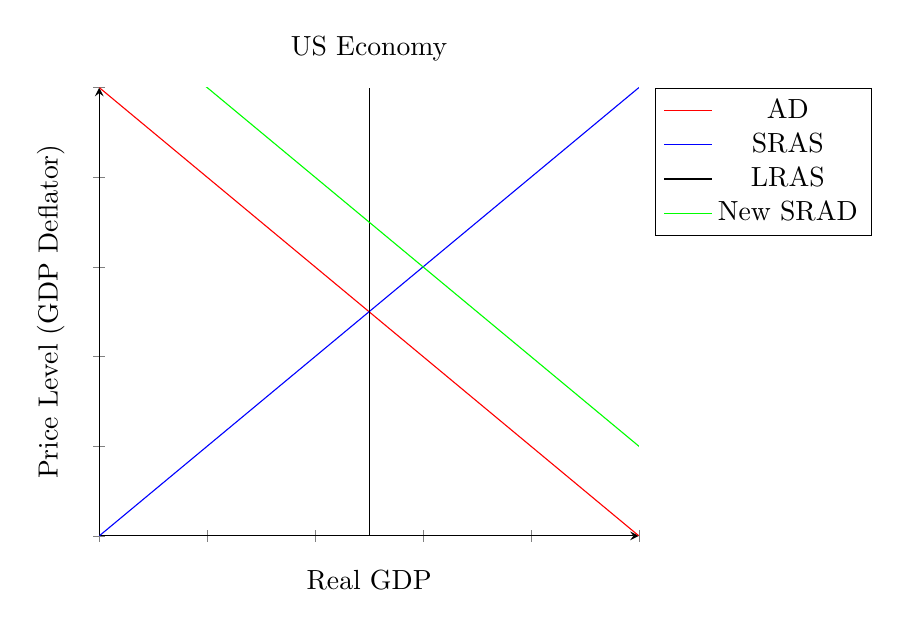
\begin{tikzpicture}
        \begin{axis}[
            title={US Economy},
            ylabel={Price Level (GDP Deflator)},
            xlabel={Real GDP},
            xmin=0, xmax=100,
            ymin=0, ymax=100,
            yticklabels={,,},
            xticklabels={,,},
            axis lines=left,
            grid=none,
            legend pos=outer north east,
        ]

        \addplot[
            color=red,
            ]
            coordinates {
            (0,100)(100,0)
            };
        \addlegendentry{AD}


        \addplot[
            color=blue,
            ]
            coordinates {
            (0,0)(100,100)
            };

        \addlegendentry{SRAS}

        \addplot[
            color=black,
            ]
            coordinates {
            (50,0)(50,100)
            };
        \addlegendentry{LRAS}

        \addplot[
            color=green,
            ]
            coordinates {
            (0,120)(120,0)
            };
        \addlegendentry{New SRAD}

        \end{axis}
    \end{tikzpicture}


    Since consumer confidence has increased, the aggregate demand curve shifts to the right. This will lead to an increase in the price level and real GDP causing increased inflation and economic growth.


    \item Would this event create an output gap? If so, what kind? Indicate this on your graph.
    
    Yes this event would create an output gap. This would be a positive output gap. This is indicated by the fact that the short-run aggregate supply curve is to the left of the long-run aggregate supply curve.


    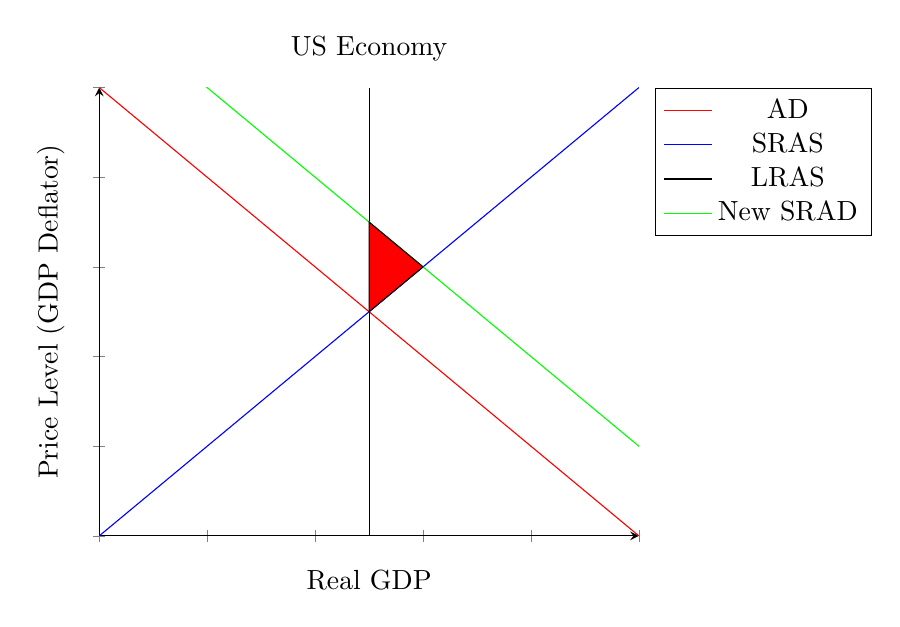
\begin{tikzpicture}
        \begin{axis}[
            title={US Economy},
            ylabel={Price Level (GDP Deflator)},
            xlabel={Real GDP},
            xmin=0, xmax=100,
            ymin=0, ymax=100,
            yticklabels={,,},
            xticklabels={,,},
            axis lines=left,
            grid=none,
            legend pos=outer north east,
        ]

        \addplot[
            color=red,
            ]
            coordinates {
            (0,100)(100,0)
            };
        \addlegendentry{AD}


        \addplot[
            color=blue,
            ]
            coordinates {
            (0,0)(100,100)
            };

        \addlegendentry{SRAS}

        \addplot[
            color=black,
            ]
            coordinates {
            (50,0)(50,100)
            };
        \addlegendentry{LRAS}

        \addplot[
            color=green,
            ]
            coordinates {
            (0,120)(120,0)
            };
        \addlegendentry{New SRAD}

        \draw (50,50)[fill=red] node[anchor=north]{}
        -- (50,70) node[anchor=north]{}
        -- (60,60) node[anchor=south]{}
        -- cycle;

        \end{axis}
    \end{tikzpicture}

    \pagebreak

    \item Has this event changed long-run potential output? If so, has it shifted up, or down?
    
    No, this event has not changed long-run potential output. This is because the long-run aggregate supply curve has not shifted and the SRAD curve will eventually shift back to the right to meet the LRAS curve.

    \item How would the market move from short-run to long-run equilibrium? Visualize this on your graph.
    

    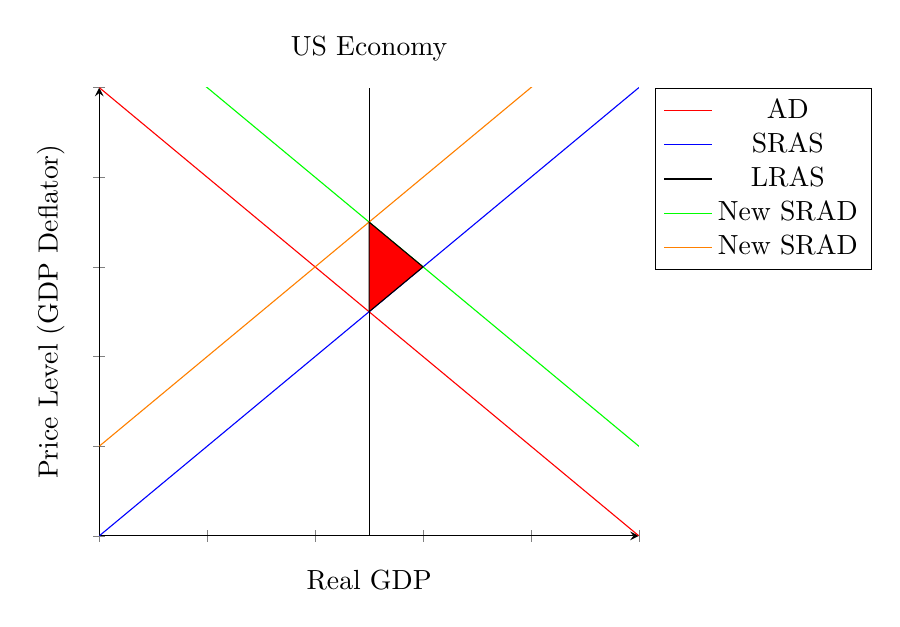
\begin{tikzpicture}
        \begin{axis}[
            title={US Economy},
            ylabel={Price Level (GDP Deflator)},
            xlabel={Real GDP},
            xmin=0, xmax=100,
            ymin=0, ymax=100,
            yticklabels={,,},
            xticklabels={,,},
            axis lines=left,
            grid=none,
            legend pos=outer north east,
        ]

        \addplot[
            color=red,
            ]
            coordinates {
            (0,100)(100,0)
            };
        \addlegendentry{AD}


        \addplot[
            color=blue,
            ]
            coordinates {
            (0,0)(100,100)
            };

        \addlegendentry{SRAS}

        \addplot[
            color=black,
            ]
            coordinates {
            (50,0)(50,100)
            };
        \addlegendentry{LRAS}

        \addplot[
            color=green,
            ]
            coordinates {
            (0,120)(120,0)
            };
        \addlegendentry{New SRAD}

        \addplot[
            color=orange,
            ]
            coordinates {
            (0,20)(100,120)
            };
        \addlegendentry{New SRAD}


        \draw (50,50)[fill=red] node[anchor=north]{}
        -- (50,70) node[anchor=north]{}
        -- (60,60) node[anchor=south]{}
        -- cycle;

        \end{axis}
    \end{tikzpicture}

    The SRAS will shift up to meet the LRAS curve. This will eventually lead to the economy returning to long-run equilibrium.

\end{enumerate}

\pagebreak

\question{3}
During the Coronavirus pandemic, U.S. policymakers used several different levers to try to limit the damage to the economy. For each of
the following policy changes, (1) decide if this was fiscal or monetary
policy, (2), specify how this policy change is designed to impact the
economy, and (3) answer the follow-up question given for each.

\begin{enumerate}[(a)]
    \item Between March 3, 2021 and March 15, 2021, the Federal Reserve announced that it would alter the discount rate (and other interest rates that it controls) in order to push the federal funds rate to 0\%.
    
    This is an example of monetary policy. The Federal Reserve is trying to stimulate the economy by lowering interest rates. This will encourage borrowing and spending, which will increase aggregate demand.

    \item The Federal Reserve also announced on March 15th that it would keep the federal funds rate near 0\% "until it is confident that the economy has weathered recent events and is on track to achieve its maximum employment and price stability goals."
    
    The Fed is engaging monetary policy to try to stabilize the economy (Forward Guidance). By setting the expectation that interest rates will remain low, the Fed is trying to encourage borrowing and spending, which will increase aggregate demand.

    \item The U.S. Congress sent taxpayers stimulus checks worth \$1,800 in 2020, and then \$1,200 in 2021.
    
    This is an example of fiscal policy. The government is trying to stimulate the economy by giving people money to spend. This will increase aggregate demand.

    \item The federal government expanded unemployment insurance in the U.S., increasing the length of time that individuals could receive unemployment insurance and also increasing the amount of money that people could receive via unemployment insurance.
    
    This is an example of fiscal policy. By increasing the amount of money that people can receive via unemployment insurance, the government is trying to increase aggregate demand.
\end{enumerate}

\pagebreak

\question{4}

Robert is thinking about taking a vacation to Europe this summer, to
visit old friends in Germany and Austria. Since these countries use
the Euro for currency, Robert will need to purchase some Euros (€)
with dollars.

\begin{enumerate}[(a)]
    \item What is the exchange rate between dollars and Euros as of October 27th, 2023?
    
    The exchange rate between dollars and Euros is 1.06 dollars per Euro.

    \item If Robert wants to purchase 1,000 €, how much will it cost him in dollars?
    
    1,060 dollars.

    \item Now consider the daily market for Euros. Given the information you found in (a), graph the market for Euros. Be sure to specify the price in this market. Assume that around 1 billion Euros are purchased each day using dollars.
    
    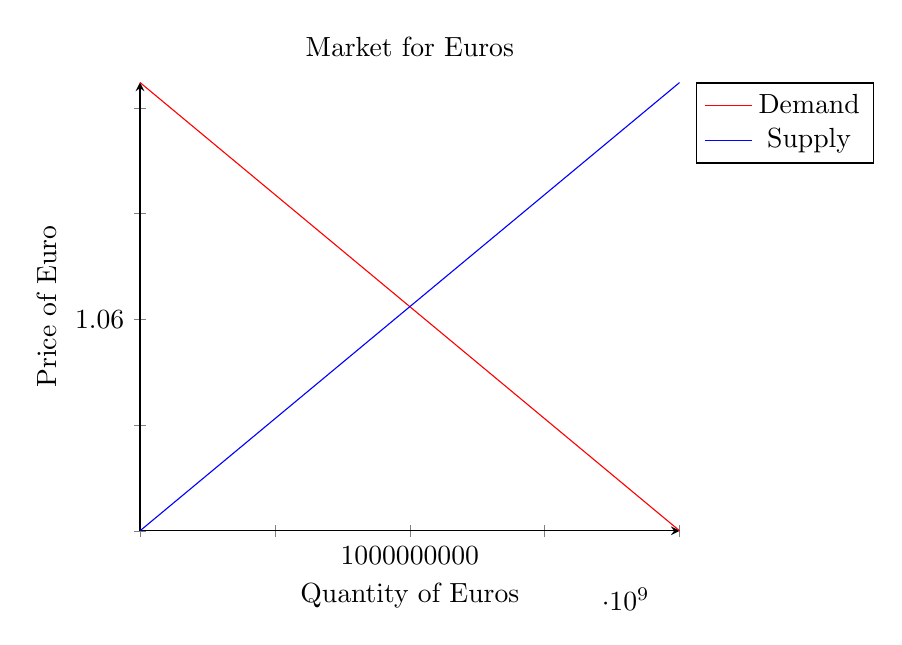
\begin{tikzpicture}
        \begin{axis}[
            title={Market for Euros},
            ylabel={Price of Euro},
            xlabel={Quantity of Euros},
            xmin=0, xmax=2000000000,
            ymin=0, ymax=2.12,
            yticklabels={0,,,1.06},
            xticklabels={0,,,1000000000},
            axis lines=left,
            grid=none,
            legend pos=outer north east,
        ]

        \addplot[
            color=red,
            ]
            coordinates {
            (0,2.12)(2000000000,0)
            };
        \addlegendentry{Demand}

        \addplot[
            color=blue,
            ]
            coordinates {
            (0,0)(2000000000,2.12)
            };
        \addlegendentry{Supply}

        \end{axis}
    \end{tikzpicture}

    \pagebreak
    \item Imagine that many, many Americans have the same idea as Robert to vacation in Europe this summer, so that the demand for Euros increases. Graph how this change will impact the market for Euros. Be sure to indicate how the price and quantity of Euros being traded for dollars is changing.
    
    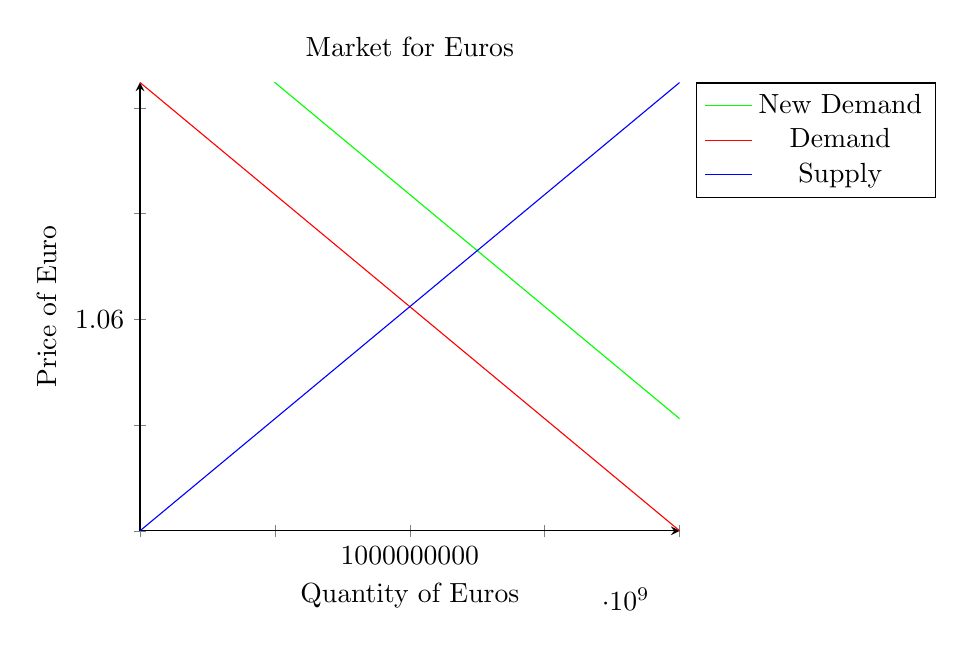
\begin{tikzpicture}
        \begin{axis}[
            title={Market for Euros},
            ylabel={Price of Euro},
            xlabel={Quantity of Euros},
            xmin=0, xmax=2000000000,
            ymin=0, ymax=2.12,
            yticklabels={0,,,1.06},
            xticklabels={0,,,1000000000},
            axis lines=left,
            grid=none,
            legend pos=outer north east,
        ]

        \addplot[
            color=green,
            ]
            coordinates {
            (0,2.65)(2500000000,0)
            };
        \addlegendentry{New Demand}

        \addplot[
            color=red,
            ]
            coordinates {
            (0,2.12)(2000000000,0)
            };
        \addlegendentry{Demand}

        \addplot[
            color=blue,
            ]
            coordinates {
            (0,0)(2000000000,2.12)
            };
        \addlegendentry{Supply}


        \end{axis}
    \end{tikzpicture}

    This would lead to an increase in the demand for Euros, which would lead to an increase in the price and quantity of Euros traded.

    \item Explain how the change in the price of a Euro will lead the quantity of Euros supplied to change.
    
    With the value of Euros compared to dollars increasing, those with Euros will be more willing to trade their Euros for dollars. This will lead to an increase in the quantity of Euros supplied.
\end{enumerate}

\pagebreak

\question{5}

The U.S. produces some computer graphics chips domestically, but
imports most of them from abroad. Assume that the world market for
graphics chips is competitive and that the U.S. is a small producer,
unable to affect the world price. The world price for computer graphics
chips is \$500. Since the U.S. imports graphics chips, we know that
in the absence of trade, the U.S. equilibrium price on graphics chips
would exceed the world price. Specifically, in the absence of trade, the
equilibrium price for a graphics chip in the U.S. would be \$600.

\begin{enumerate}[(a)]
    \item Draw a diagram showing the U.S. market for graphics chips, given the world market for graphics chips that the U.S. can access.
    
    Diagram drawn.

    \item On your graph above, indicate where we can see the U.S. production of graphics chips, and where we can see the quantity of graphics chips being imported.
    

    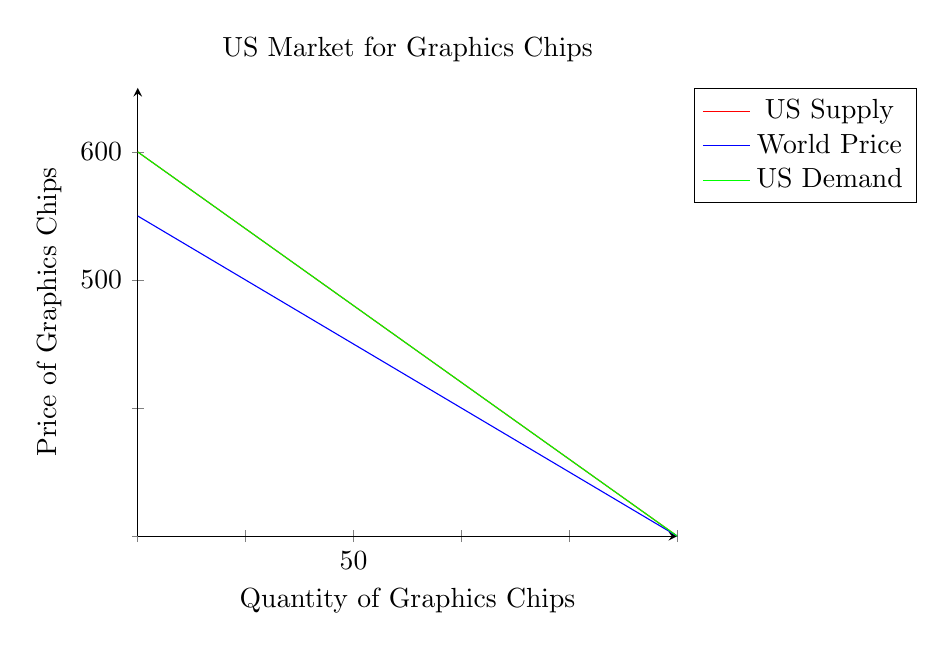
\begin{tikzpicture}
        \begin{axis}[
            title={US Market for Graphics Chips},
            ylabel={Price of Graphics Chips},
            xlabel={Quantity of Graphics Chips},
            xmin=0, xmax=100,
            ymin=0, ymax=700,
            yticklabels={0,,,500,600},
            xticklabels={0,,,50},
            axis lines=left,
            grid=none,
            legend pos=outer north east,
        ]

        \addplot[
            color=red,
            ]
            coordinates {
            (0,600)(100,0)
            };
        \addlegendentry{US Supply}

        \addplot[
            color=blue,
            ]
            coordinates {
            (0,500)(100,0)
            };
        \addlegendentry{World Price}

        \addplot[
            color=green,
            ]
            coordinates {
            (0,600)(100,0)
            };
        \addlegendentry{US Demand}

        \end{axis}
    \end{tikzpicture}

    
    \item Assuming they are identical in terms of capabilities, will the domestically produced graphics chips sell for the same price as the imported ones? Why or why not?
    
    No, the domestically produced graphics chips will sell for a higher price than the imported ones. This is because the world price for graphics chips is lower than the equilibrium price in the U.S. Without trade, the price of graphics chips in the U.S. would be \$600. Since the world price is \$500, the domestically produced graphics chips will sell for a higher price than the imported ones.

    \item Imagine that the U.S. imposes a \$50 tariff on graphics chips. Graph the impact of this tariff on the U.S. market. Indicate where we can see the domestic production of graphics chips, as well as any imported graphics chips (if any are still imported).
    
    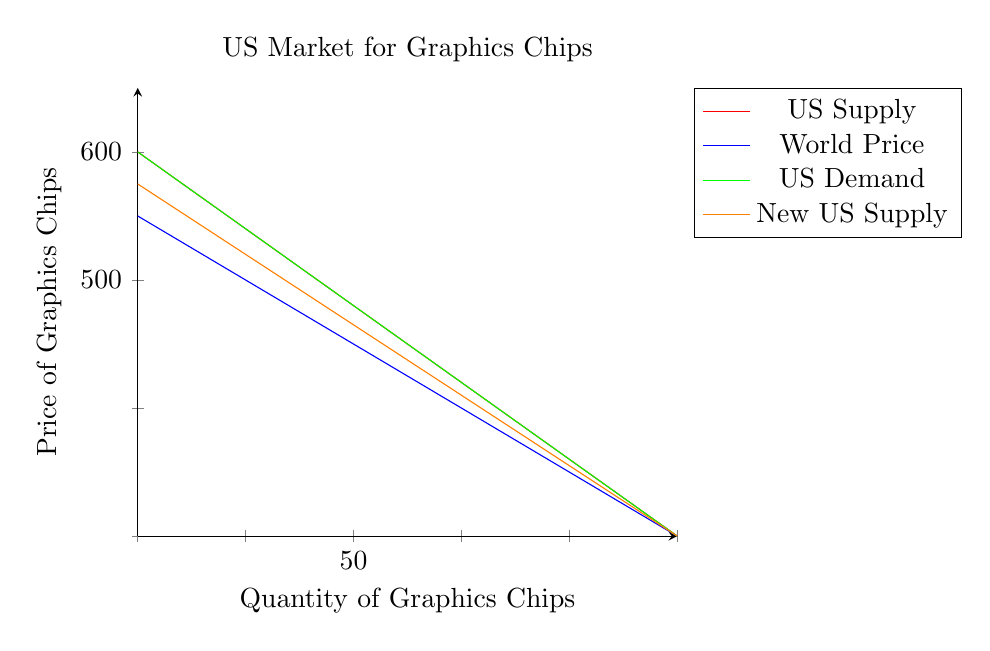
\begin{tikzpicture}
        \begin{axis}[
            title={US Market for Graphics Chips},
            ylabel={Price of Graphics Chips},
            xlabel={Quantity of Graphics Chips},
            xmin=0, xmax=100,
            ymin=0, ymax=700,
            yticklabels={0,,,500,600},
            xticklabels={0,,,50},
            axis lines=left,
            grid=none,
            legend pos=outer north east,
        ]

        \addplot[
            color=red,
            ]
            coordinates {
            (0,600)(100,0)
            };
        \addlegendentry{US Supply}

        \addplot[
            color=blue,
            ]
            coordinates {
            (0,500)(100,0)
            };
        \addlegendentry{World Price}

        \addplot[
            color=green,
            ]
            coordinates {
            (0,600)(100,0)
            };
        \addlegendentry{US Demand}

        \addplot[
            color=orange,
            ]
            coordinates {
            (0,550)(100,0)
            };
        \addlegendentry{New US Supply}

        \end{axis}
    \end{tikzpicture}

    \item Including the cost of the tariff, how will the cost of a U.S. graphics chip compare to the cost of an imported graphics chip? Explain your answer.
    
    The cost of a U.S. graphics chip will be higher than the cost of an imported graphics chip. This is because the tariff will increase the price of the U.S. graphics chip by \$50. This will make the U.S. graphics chip more expensive than the imported graphics chip.

    \item Who benefits and who is harmed by such a tariff? Show these effects in your diagram.
    
    The U.S. producers of graphics chips benefit from the tariff. This is because the tariff increases the price of the U.S. graphics chips, which will increase their revenue. The U.S. consumers of graphics chips are harmed by the tariff. This is because the tariff increases the price of the U.S. graphics chips, which will increase the cost of the graphics chips for U.S. consumers.
\end{enumerate}

\end{document}